\chapter{Background}

In this chapter, topics such as citizen science, gamification, and speech corpus will be further described. Additional terms relevant to the research will also be defined and clarified, to ensure all research topics are clear. 

\section{Citizen Science}

\subsection{Origins}

According to \cite{asd}, citizen science originates from two sources.

\subsection{Definition}

The term citizen science.

\subsection{Classifications}

Below are some classifications in which citizen science projects can be divided:

\subsubsection{Volunteer Involvement}

An initial classification based on volunteer involvement \cite{follett2015analysis}: 
\begin{itemize}
    \item Contributory, where participants contribute to data collection and sometimes help analyze and disseminate results
    \item Collaborative, where citizens also analyze samples, design the study, interpret the data, draw conclusions and disseminate results
    \item Co-created, where they participate in all stages of the project, including defining questions, developing hypotheses, drawing conclusions, discussing results and answering new questions
\end{itemize}

\subsubsection{Goals of the study}

An alternative classification for these initiatives has been suggested by \cite{wiggins2011conservation}, and is based on the goals of the study:

\begin{itemize}
    \item Action projects, initiated by volunteers designed to encourage intervention in local concerns;
    \item Conservation projects, addressing natural resource management goals;
    \item Investigation projects, focusing on scientific research goals in a physical setting;
    \item Virtual projects, also focusing on scientific goals, but entirely based on information technology with all volunteer interaction occurring online;
    \item Education projects; often performed in the classroom or school grounds as part of the science curriculum.
\end{itemize}

\subsubsection{Topic of study}

An additional way of classifying citizen science projects is based on the topic of study, for example, astronomy, archaeology, and biology \cite{wiggins2011conservation}. 

\subsubsection{This work}

If these classifications are to be applied in this work, it should be categorized as a \textbf{contributory virtual speech corpus} citizen science project.

\subsection{Relevant Virtual Projects}

With the recent growth of citizen science, various breakthroughs were made possible. Below are some of the most relevant projects in the virtual space.

\subsubsection{Foldit}

\begin{figure}[ht]
    \centering
    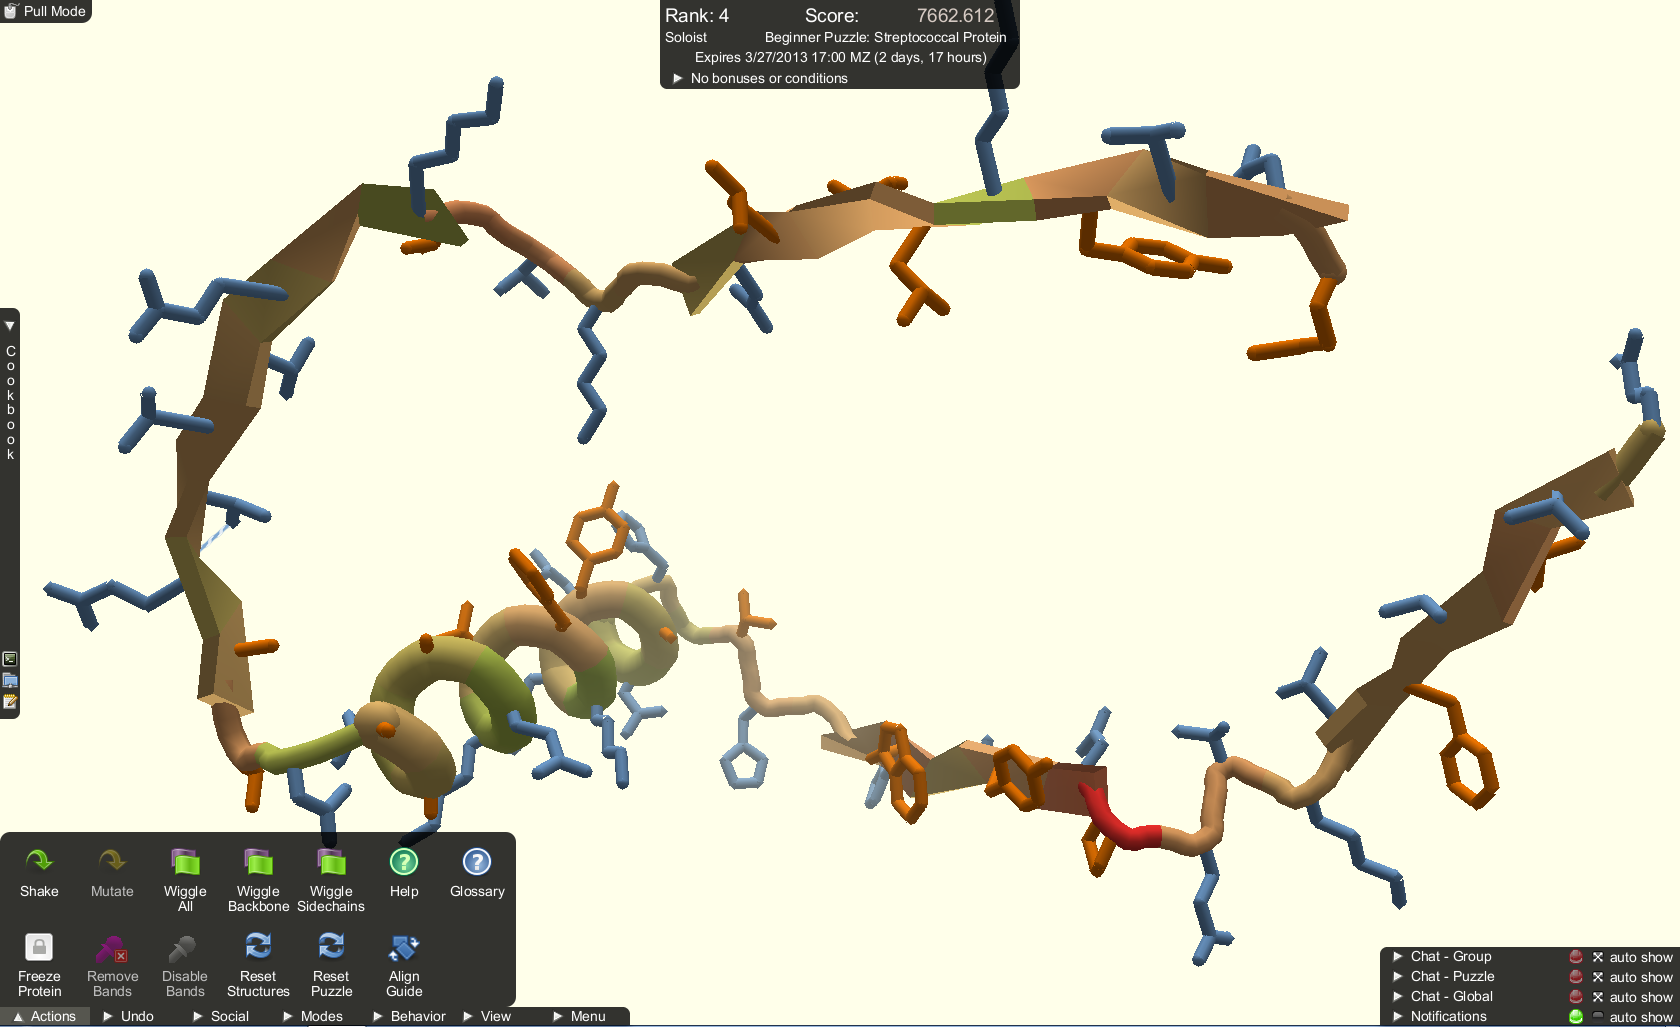
\includegraphics[width=\linewidth]{images/background/foldit-problem.png}
    \caption{Foldit - Unfolded (and unstable) Streptococcal Protein Puzzle \\ Source: \cite{foldit-protein-problem}}
    \label{fig:foldit-problem}
\end{figure}

Foldit, designed by researchers at the University of Washington, is a game in which gamers solve protein folding patterns, a central challenge in biochemistry, by virtually wiggling, shaking and pulling shapes to create small stable structures, as well as developing their own algorithms for solving protein folding \cite{bourzac2008enlisting}. 

\begin{figure}[ht]
    \centering
    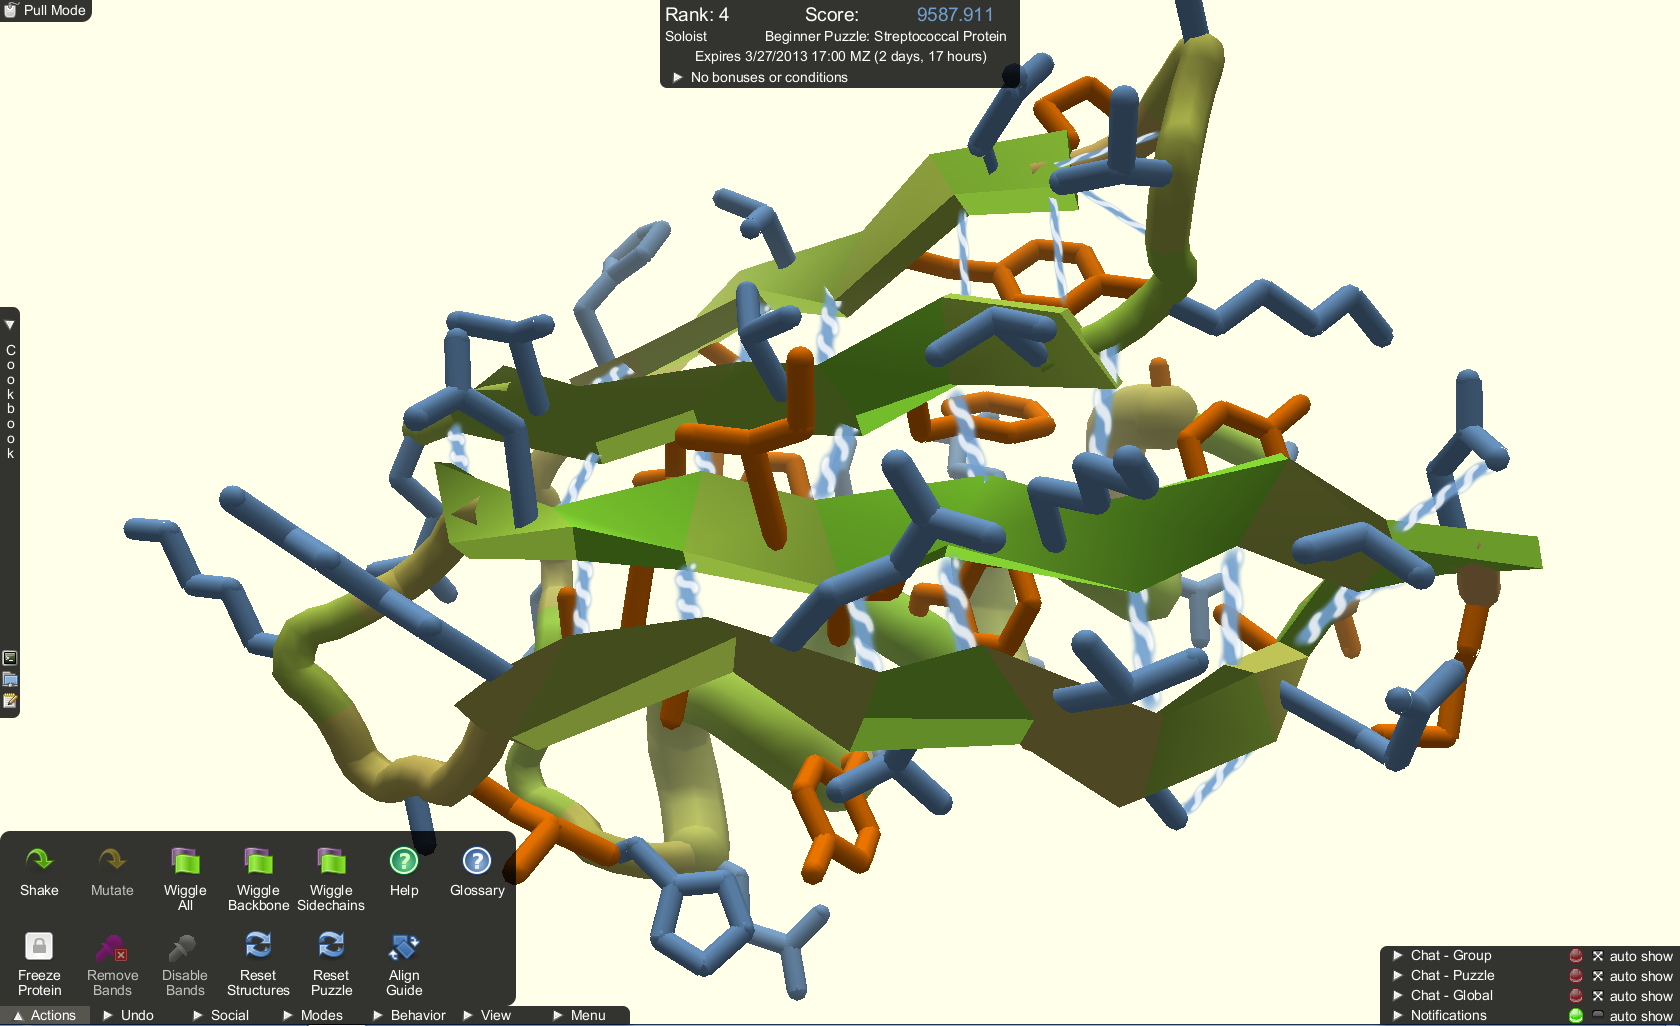
\includegraphics[width=\linewidth]{images/background/foldit-solution.png}
    \caption{Foldit - Folded up Streptococcal Protein Puzzle \\ Source: \cite{foldit-protein-solution}}
    \label{fig:foldit-solution}
\end{figure}

As the moment of this article, Foldit has had 20 peer-reviewed articles in a number of journals and conferences \cite{foldit-publications}. Some relevant breakthroughs are a potential target for HIV drug development \cite{khatib2011crystal}, redesign of the catalyst for the Diels-Alder reaction \cite{eiben2012increased}, and improvement of cryo-electron microscopy atomic model building and refinement \cite{khatib2019building}.

\begin{table}[h]
    \centering
    \begin{tabular}{|c|c|c|}
        \hline Project & Contributors & Contributions \\
        \hline Foldit & access & access \\ 
        \hline EyeWire & access & access \\ 
        \hline Galaxy Zoo & access & access \\ 
        \hline Christmas Audubom Birdwatch & access & access \\ \hline 
    \end{tabular}
    \caption{Contribution for online citizen science projects}
    \label{tab:cs-contributions}
\end{table}

\subsubsection{Zooniverse}

\begin{figure}[ht]
    \centering
    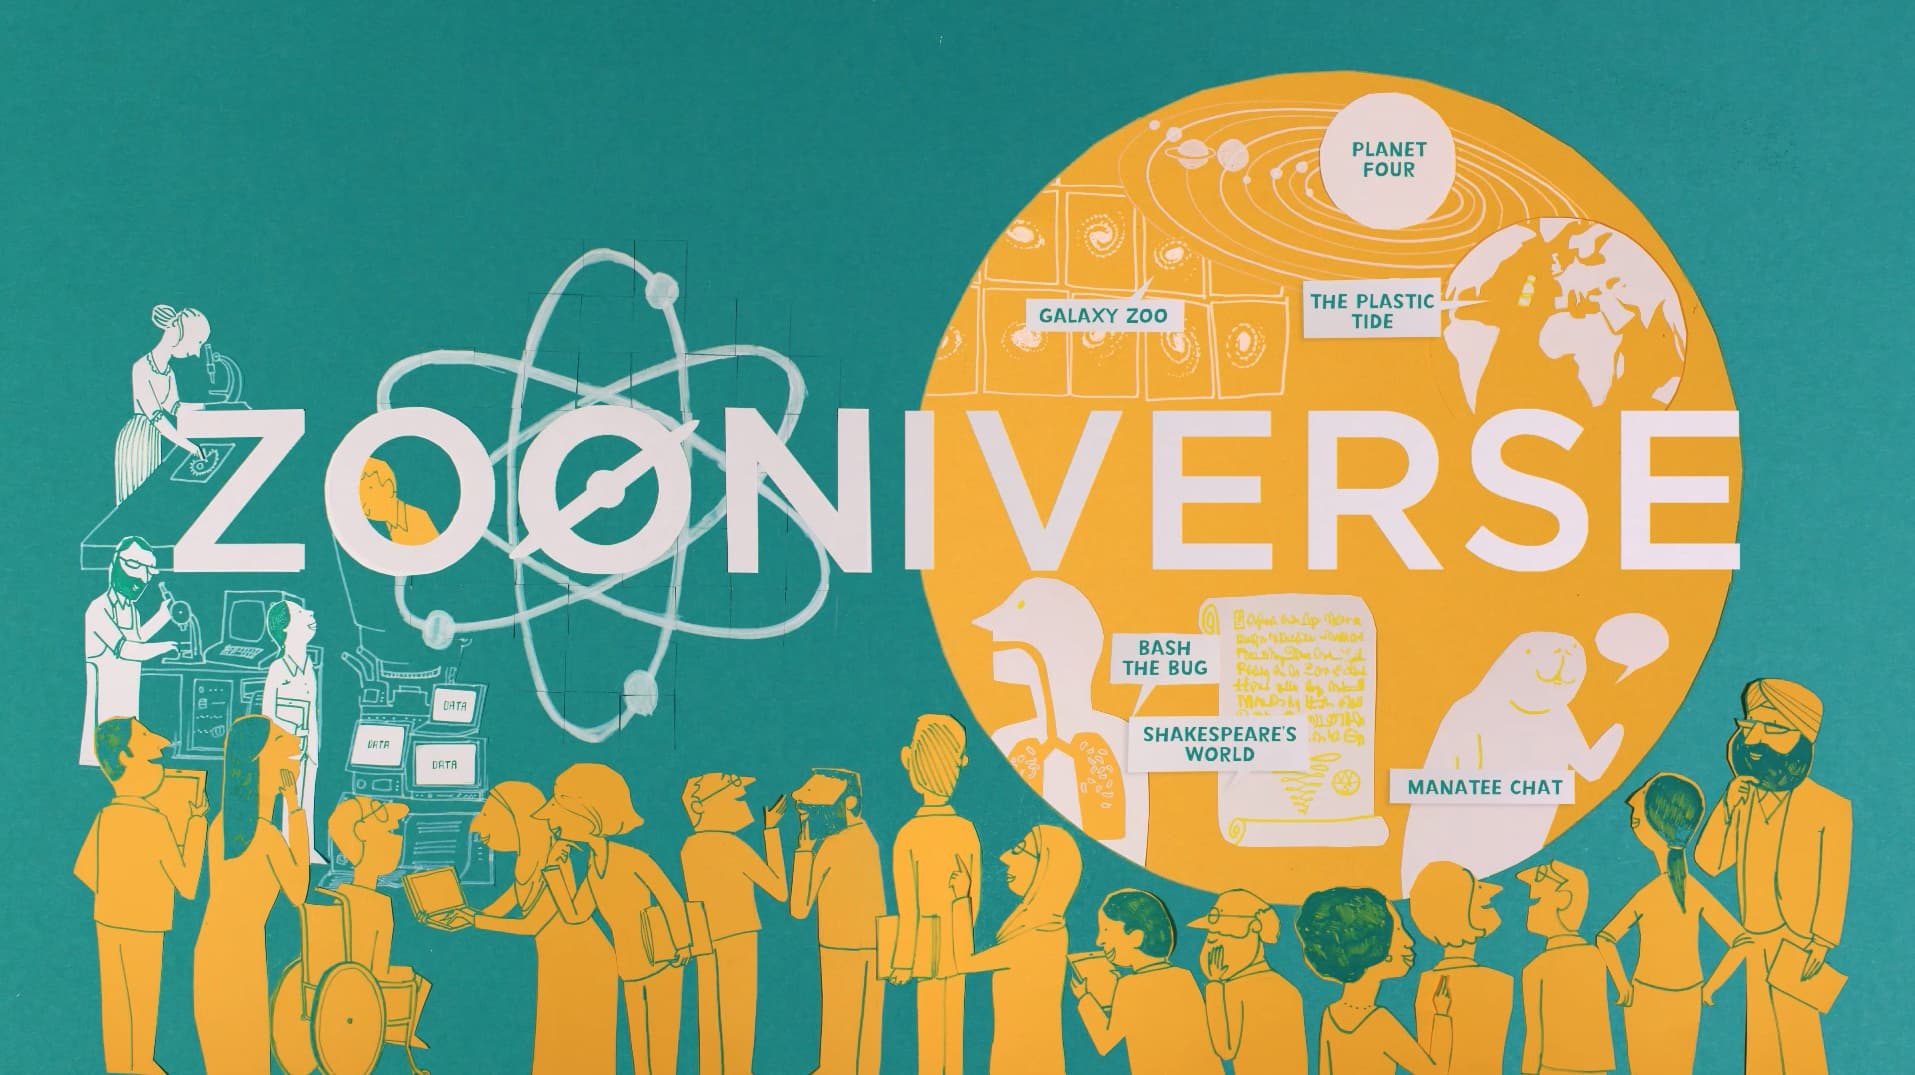
\includegraphics[width=\linewidth]{images/background/zooniverse.jpg}
    \caption{Zooniverse Platform, connecting volunteers with scientists \\ Source: \cite{zooniverse-logo}}
    \label{fig:foldit-solution}
\end{figure}

Zooniverse is a platform for citizen science projects. It connects more than a million volunteers around the world to assist professional researchers. The platform has a simple interface for input and classification of data, as well as the creation and management of projects.

This collaborative platform has enabled over 300 of scientific publications, with publications from the (1) discovery and classification of stars, planets, supernovas; humanities, animal identification, classification of whale calls, datasets etc.

\subsubsection{Galaxy Zoo}

https://www.zooniverse.org/projects/zookeeper/galaxy-zoo

\subsection{Ten Principles of Citizen Science}

According to the European Citizen Science Association, citizen science is a flexible concept which can be adapted and applied within diverse situations and disciplines. The association set out some key principles which as a community they believe underlie good practice in citizen science. Appendix \ref{app:ten-principles} lists all ten principles.

\section{Gamification}

\subsection{Crowdfunding}

\section{Natural Language Processing}

\subsection{Speech Recognition}

\section{Speech Corpus}

\section{Systematic Literature Review}

